\documentclass[11pt, a4paper]{article}
\usepackage[utf8]{inputenc}
\usepackage{amsmath, amssymb}
\usepackage{graphicx}
\usepackage{hyperref}
\usepackage{geometry}
\geometry{margin=1in}

\title{EE 325 Digital Signal Processing \\ Assignment 4: z-Transform and Inverse z-Transform}
\author{PERERA J.D.T. \\ E/21/291}
\date{\today}

\begin{document}
\maketitle

\section{1. Forward z-Transform}
\textbf{Question:} Find the z-transform $X(z)$ and region of convergence (ROC) of $x[n] = 0.5^n u[n]$.

\textbf{Solution:}
The definition of the z-transform is:
$$X(z) = \sum_{n=-\infty}^{\infty} x[n] z^{-n}$$

Substituting $x[n]$:
$$X(z) = \sum_{n=0}^{\infty} 0.5^n z^{-n} = \sum_{n=0}^{\infty} (0.5 z^{-1})^n$$

This is a geometric series of the form $\sum_{n=0}^{\infty} r^n = \frac{1}{1-r}$, which converges if $|r| < 1$.
Here, $r = 0.5z^{-1}$.

Convergence condition:
$$|0.5 z^{-1}| < 1 \implies \frac{0.5}{|z|} < 1 \implies |z| > 0.5$$

Result:
$$X(z) = \frac{1}{1 - 0.5z^{-1}} = \frac{z}{z - 0.5}$$

\textbf{ROC:} $|z| > 0.5$

\section{2. Inverse z-Transform by Partial Fractions}
\textbf{Question:} Given $X(z) = \frac{2z}{(z-1)(z+0.5)}$ and assuming valid causal $x[n]$, find $x[n]$.

\textbf{(a) Partial Fraction Expansion:}
We expand $\frac{X(z)}{z}$ to easily handle the roots:
$$\frac{X(z)}{z} = \frac{2}{(z-1)(z+0.5)} = \frac{A}{z-1} + \frac{B}{z+0.5}$$

finding A:
$$A = \left. \frac{2}{z+0.5} \right|_{z=1} = \frac{2}{1.5} = \frac{4}{3}$$

finding B:
$$B = \left. \frac{2}{z-1} \right|_{z=-0.5} = \frac{2}{-1.5} = -\frac{4}{3}$$

So,
$$\frac{X(z)}{z} = \frac{4/3}{z-1} - \frac{4/3}{z+0.5}$$
$$X(z) = \frac{4}{3} \frac{z}{z-1} - \frac{4}{3} \frac{z}{z+0.5}$$

\textbf{(b) Time-domain sequence x[n]:}
Using standard transform pairs for causal sequences ($|z| > 1$):
$$\frac{z}{z-a} \longleftrightarrow a^n u[n]$$

Term 1: $\frac{4}{3} (1)^n u[n]$ \\
Term 2: $-\frac{4}{3} (-0.5)^n u[n]$

$$x[n] = \frac{4}{3} u[n] - \frac{4}{3} (-0.5)^n u[n]$$
$$x[n] = \frac{4}{3} [1 - (-0.5)^n] u[n]$$

\textbf{(c) Sketch and Decay:}
\begin{itemize}
    \item For $n=0$: $x[0] = 4/3(1 - 1) = 0$
    \item For $n=1$: $x[1] = 4/3(1 - (-0.5)) = 4/3(1.5) = 2$
    \item For $n \to \infty$: $(-0.5)^n \to 0$, so $x[n] \to 4/3 \approx 1.33$
\end{itemize}

The system has a transient response due to the pole at $-0.5$ (alternating decay) and a steady-state response due to the pole at $1$ (step).

\section{3. Python Verification}
The symbolic result matches the analytical result perfectly. Programmatically derived:
$$x[n] = 1.333 \cdot 1^n - 1.333 \cdot (-0.5)^n$$

\begin{figure}[h]
    \centering
    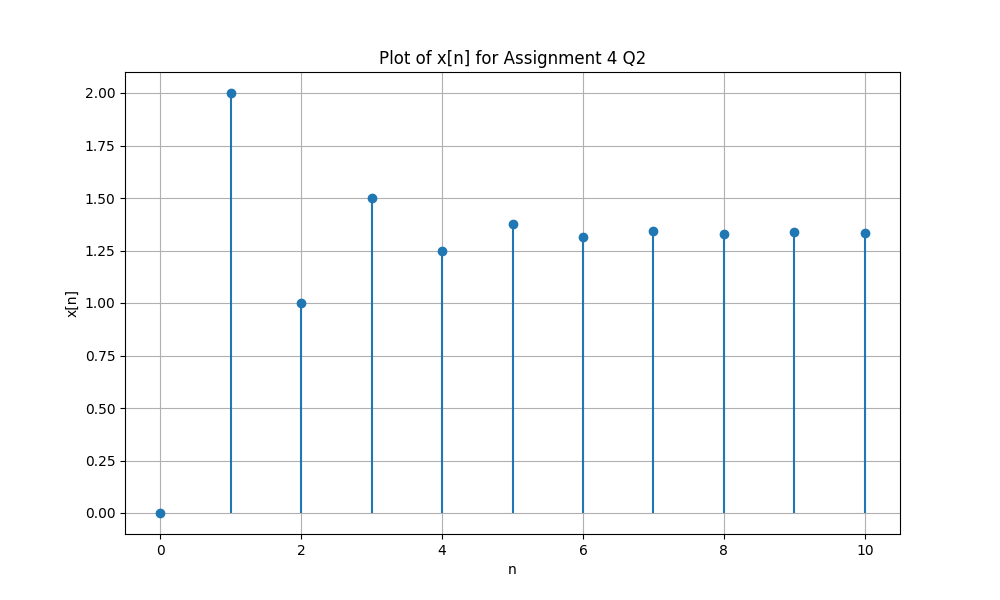
\includegraphics[width=0.8\textwidth]{x_n_plot.png}
    \caption{Plot of time-domain sequence $x[n]$}
    \label{fig:xn_plot}
\end{figure}

\end{document}
